\begin{pa} \label{PA:10.4} 
  Let's consider the function 
  $$
  f(x,y) = 6 - \frac{x^2}2 - y^2,
  $$
  whose graph is shown in Figure \ref{F:10.4.tangent.1}.  

  \begin{figure}[ht]
    \begin{center}
      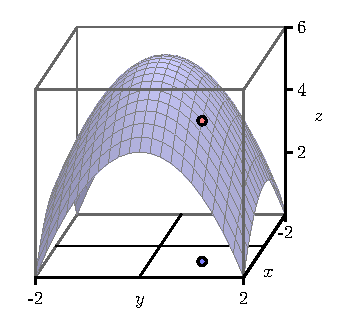
\includegraphics{figures/fig_10_4_tangent_1.eps}
    \end{center}
    \caption{The graph of $f(x,y)=6-x^2/2 - y^2$.}
    \label{F:10.4.tangent.1}
  \end{figure}

  We will study the behavior of this function near the point $(x_0,
  y_0) = (1,1)$.  In particular, we wish to view the graph on an
  increasingly small scale around this point, as shown in Figure
  \ref{F:10.4.tangent.2} 

  \begin{figure}[ht]
    \begin{center}
      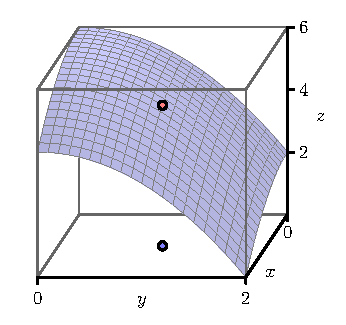
\includegraphics{figures/fig_10_4_tangent_2.eps}
      \hspace*{20pt}
      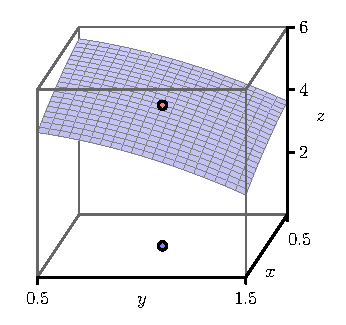
\includegraphics{figures/fig_10_4_tangent_3.eps}
    \end{center}
    \caption{The graph of $f(x,y)=6-x^2/2 - y^2$.}
    \label{F:10.4.tangent.2}
  \end{figure}

  Just as the graph of a single-variable function looks like a line
  when viewed on a small scale, we see that the graph of a
  two-variable function looks like a plane, as seen in Figure
  \ref{F:10.4.tangent.4}.  We wish to write the equation of this
  line. 

  \begin{figure}[ht]
    \begin{center}
      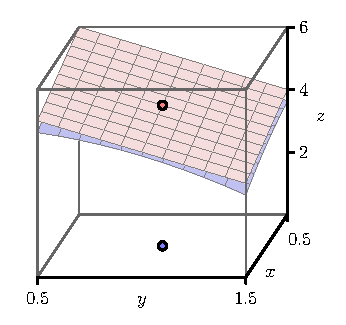
\includegraphics{figures/fig_10_4_tangent_4.eps}
    \end{center}
    \caption{The graph of $f(x,y)=6-x^2/2 - y^2$.}
    \label{F:10.4.tangent.4}
  \end{figure}

  Remember that in Section \ref{S:9.5.Lines_Planes}, we saw that the
  equation of a plane passing through the point $(x_0, y_0, z_0)$
  could be written as $A(x-x_0) + B(y-y_0) + C(z-z_0) = 0$.  If the
  plane is not vertical, then $C\neq 0$, and we can
  rearrange this as
  \begin{align*}
    C(z-z_0) & = -A(x-x_0) - B(y-y_0) \\
    z & = z_0-\frac AC(x-x_0) - \frac BC(y-y_0) \\
    z & = z_0 + a(x-x_0) + b(y-y_0)
  \end{align*}
  where we have written the constants $-A/C$ and $-B/C$ as $a$ and
  $b$, respectively.
    
\ba
\item Remember that we are focusing on the point $(x_0,y_0) = (1,1)$.
  Evaluate the function $f(1,1)$ and its partial derivatives
  $f_x(1,1)$ and $f_y(1,1)$.

\item We know one point on the tangent plane;  namely, the tangent
  plane agrees with the graph of the function at the point $(x_0,
  y_0)$.  Use this observation to determine $z_0$ in the expression
  $z = z_0 + a(x-x_0) + b(y-y_0)$.

\item Sketch the traces of the function for $y=y_0=1$ and $x=x_0=1$
  below in Figure \ref{F:10.4.traces}.  

  \begin{figure}[ht]
    \begin{center}
      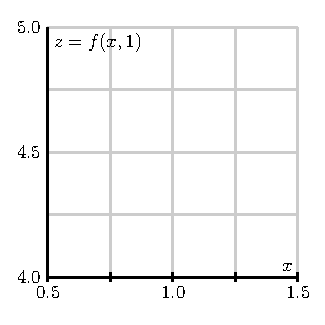
\includegraphics{figures/fig_10_4_tangent_trace_y.eps}
      \hspace*{20pt}
      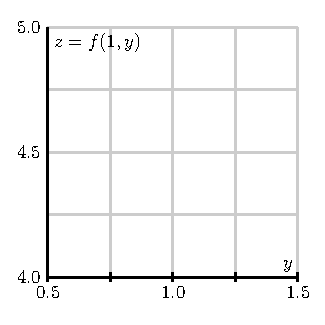
\includegraphics{figures/fig_10_4_tangent_trace_x.eps}
    \end{center}
    \caption{The traces of $f(x,y)$ with $y=y_0=1$ and $x=x_0=1$.}
    \label{F:10.4.traces}
  \end{figure}

\item Write the equation of the tangent line of the trace with $y=1$
  at the point $x_0=1$.  

\item Figure \ref{F:10.4.tangent.traces} shows the traces of the
  function and the traces of the tangent plane.  How does your work in
  the last part of this activity tell you the equation of the trace of
  the tangent plane with $y=1$?

  \begin{figure}[ht]
    \begin{center}
      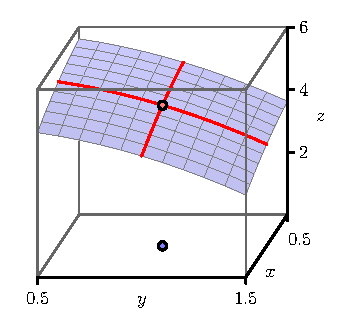
\includegraphics{figures/fig_10_4_tangent_5.eps}
      \hspace*{20pt}
      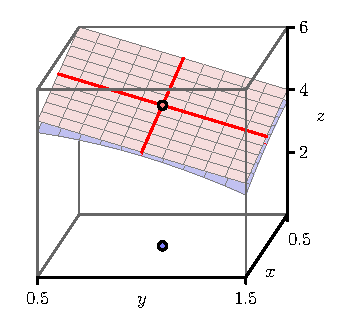
\includegraphics{figures/fig_10_4_tangent_6.eps}
    \end{center}
    \caption{The traces of $f(x,y)$ and the tangent plane.}
    \label{F:10.4.tangent.traces}
  \end{figure}

\item Using 





  \ea



\end{pa} \afterpa 